\documentclass[fleqn]{article}

\usepackage[margin=2.5cm, headheight=23pt]{geometry}
\usepackage{graphicx}
\usepackage{mathtools}
\usepackage{amsmath}
\usepackage{amsfonts}
\usepackage{colortbl}
\usepackage{empheq}
\usepackage[shortlabels]{enumitem}
\usepackage{color}

\usepackage{hyperref}
\hypersetup{
  colorlinks=true,
  linkcolor=blue,
  urlcolor=blue
}

\usepackage{caption}
%\captionsetup[figure]{labelformat=empty}
\usepackage{subcaption}
%\captionsetup[subfigure]{labelformat=empty}



\definecolor{dkgreen}{rgb}{0,0.6,0}
\definecolor{gray}{rgb}{0.5,0.5,0.5}
\definecolor{mauve}{rgb}{0.58,0,0.82}
\definecolor{mauve}{rgb}{1.0,0,0}


\title{HSE Setup and Usage Guide}
\author{Robert Jans}


\begin{document}

\setlength{\parindent}{0cm}

\maketitle

\newpage

\hypersetup{
  linkcolor=black
}
\tableofcontents
\hypersetup{
  linkcolor=blue
}

\newpage

%%%%%%%%%%%%%%%%%%%%%%%%%%%%%%%%%%%%%%%%%%%%%%%%%%%%%%%%%%%%%%%%%%%%%%%%%%%%%
\section{(Temporary) Source Download and Running Application}
%%%%%%%%%%%%%%%%%%%%%%%%%%%%%%%%%%%%%%%%%%%%%%%%%%%%%%%%%%%%%%%%%%%%%%%%%%%%%

The source codes and related documentation files are available on \emph{GitHub} under \\

\href{https://github.com/robix82/bsc_project/}{https://github.com/robix82/bsc\_project/}. \\

The repository can be cloned by issuing the following command 
\begin{verbatim}
git clone https://github.com/robix82/bsc_project.git
\end{verbatim}

For testing the application and its interactions with Qualtrics, I temporarily deployed it on \\

\url{http://www.robix-projects.org/hse}. \\


You can log in using the following credentials;

\begin{itemize}
\item username: admin
\item password: admin
\end{itemize}

%%%%%%%%%%%%%%%%%%%%%%%%%%%%%%%%%%%%%%%%%%%%%%%%%%%%%%%%%%%%%%%%%%%%%%%%%%%%%
\section{Employed Technologies}
%%%%%%%%%%%%%%%%%%%%%%%%%%%%%%%%%%%%%%%%%%%%%%%%%%%%%%%%%%%%%%%%%%%%%%%%%%%%%

The project is constructed as a web application using the \emph{SpringBoot} framework. It consists in 
a back-end written in java, HTMl pages (served via the \emph{Thymeleaf} templating engine), some
\emph(JavaScript) to be run on client side, and \emph{css} files for the user interface styling. 
Data is stored in part in a \emph{MySql} database and in part as text files
on the server's file system. The \emph{JQuery} and \emph{Bootstrap} frameworks are used for keeping the
front-end code as simple as possible.

Dependency management and build configurations are handled by the \emph{Maven} project management tool.
In order to allow a simple deployment procedure, the application is packaged into a \emph{Docker} image
at build time. The application can be started and stopped using \emph{Docker Compose} which automatically
downloads, initializes, and links the required \emph{MySql} database.
For a detailed deployment description, see section~\ref{sec:deployment}. 
For inspecting and/or modifying the source code, I suggest using the \emph{Eclipse} IDE.

%%%%%%%%%%%%%%%%%%%%%%%%%%%%%%%%%%%%%%%%%%%%%%%%%%%%%%%%%%%%%%%%%%%%%%%%%%%%%%%%%%%%%%
\section{Configuration, Build and Deployment}
\label{sec:deployment}
%%%%%%%%%%%%%%%%%%%%%%%%%%%%%%%%%%%%%%%%%%%%%%%%%%%%%%%%%%%%%%%%%%%%%%%%%%%%%%%%%%%%%%

%%%%%%%%%%%%%%%%%%%%%%%%%%%%%%%%%%%%%%%%%%%
\subsection{Dependencies}

The system on which you build the application must have the following software installed:

\begin{itemize}

\item Java JDK 11

\item Apache Maven 3.6.3

\item Docker version 20.10.1

\end{itemize}

If you need to run the application locally without using docker, also \emph{MySql} is required. 

The server on which the application is to be deployed, only needs \emph{Docker} and \emph{Docker Compose}.

%%%%%%%%%%%%%%%%%%%%%%%%%%%%%%%%%%%%%%%%%%%
\subsection{Configuration Files}

\subsubsection{Maven configuration: pom.xml}

The build settings used by \emph{Maven} are defined in \texttt{/hse/pom.xm}. This file contains some general information
about the project, such as name and version, as well as a list of java packages and \emph{Maven} plugins which are 
downloaded and set up at build time. The File also declares two profiles (``dev'' and ``prod''). The ``dev'' profile 
is intended for creating a local build to be used during development, while the ``prod'' profile is to be used for building the deployment version.
The profiles are linked to specific configuration files which contain various settings such as server ports and global
constants: when the profile ``dev'' is selected, the application uses the file \texttt{/hse/src/main/resources/application-dev.properties};
when ``prod'' is selected, \texttt{/hse/src/main/resources/application-prod.properties}. 

By default the ``dev'' profile is selected;
for using the ``prod'' profile, the flag \texttt{-Pprod} is to be included in the \emph{Maven} command 
(e.g. \texttt{mvn -Pprod clean install}).

\subsubsection{Specific configurations in \texttt{.properties} files}

The directory \texttt{/hse/src/main/resources/} contains three files with extension \texttt{.properties}:

\texttt{application.properties}, \texttt{application-dev.properties} and \texttt{application-prod.properties}.
The first one contains settings that are applied independently of the selected profile, while the other
two contain profile-specific settings. The crucial settings to be considered at build time are the 
\texttt{spring.datasource.xxx} properties, which indicates the database which the application is going to connect to, and 
the \texttt{baseUrl} parameter, which indicates the prefix used at server level.
For instance in the \texttt{application-prod.properties} as I have set it up, the data source is pointing to a \emph{MySql} Docker container,
and the base url is set to \texttt{/hse/}, since I deploy it on \texttt{http://www.robix-projects.org/hse/}. 
In the \texttt{application-dev.properties} file the data source points to a local \emph{MySql} instance and the baseUrl is \texttt{/}.

The other properties indicate directory paths and should not need to be modified.

\subsubsection{docker-compose.yml}

The simplest way to run the application on a server is by using \emph{Docker Compose}. The way in which the containers are created from the images
and the internal ports used are defined in 
\texttt{/hse/docker-compose.yml}.

%%%%%%%%%%%%%%%%%%%%%%%%%%%%%%%%%%%%%%%%%%%
\subsection{Creating a local build}

\subsubsection{Preparing the database}

In order to run the application locally , a \emph{MySql} database service running on port 3306 is required. The service must contain a database
named \texttt{hse\_db} and should be accessible via username \texttt{root} and password \texttt{root}. The tables
are created automatically at application startup. If you need to use other login credentials, or the service is running on another port, these
parameters can be set in \texttt{application-dev.properties}.

\subsubsection{Issuing the build command}

The command
\begin{verbatim}
mvn clean install
\end{verbatim}
initiates the build process. The process involves executing several test suites, which should work without failure. In case
the tests fail (e.g. due to path incompatibilities or missing files) the tests can be skipped using the \texttt{-DskipTests} flag:
\begin{verbatim}
mvn -DskipTests clean install
\end{verbatim}

\subsubsection{Running the application}

Once the application is built, it can be run in several ways. During development it is convenient to run it from the IDE (in
\emph{Eclipse} package explorer, right-click on project $\rightarrow$ Run As $\rightarrow$ Spring Boot App). Alternatives are to run it from command
line using \emph{Maven}:
\begin{verbatim}
cd hse/
mvn spring-boot:run
\end{verbatim}
or using \emph{Java}:

\begin{verbatim}
cd hse/target/
java -jar hse-0.1.jar
\end{verbatim}

%%%%%%%%%%%%%%%%%%%%%%%%%%%%%%%%%%%%%%%%%%%
\subsection{Example deployment on \emph{Ubuntu Server} with \emph{Apache2}}

\subsubsection{Create and transfer the \emph{Docker} image}

The first step consists in creating the application's image by issuing

\begin{verbatim}
cd hse/
mvn -Pprod clean install
\end{verbatim}

At this point, the output of \texttt{docker image ls} should contain a line similar to:

\begin{verbatim}
REPOSITORY           TAG       IMAGE ID       CREATED             SIZE
robix82/usi.ch-hse   0.1       c2137e7cc110   37 seconds ago      758MB
\end{verbatim}

Once the image is created it can be exported as a \texttt{.tar} file by issuing

\begin{verbatim}
docker save robix82/usi.ch-hse:0.1 > hse.tar
\end{verbatim}

Finally the \texttt{.tar} file and \texttt{/hse/docker-compose.yml} must be copied to the server, e.g. using \texttt{scp}.

\subsubsection{Load the image and start the application}

On the server, the image from the \texttt{.tar} file can be loaded with

\begin{verbatim}
docker load < hse.tar
\end{verbatim}

With the image loaded, the application can be started by issuing

\begin{verbatim}
docker-compose up &
\end{verbatim}

from the directory containing the \texttt{docker-compose.yml} file. The required \emph{MySql} image will
be downloaded and initialized automatically.

At this point the application is reachable on port 8081 (the port can be configured in \texttt{docker-compose.yml}).

\subsubsection{Apache2 configuration}

In order to make the application reachable on the server's external address with a custom prefix, it is necessary to
configure a virtual host using Apache's \texttt{mod\_proxy} module. For details on \texttt{mod\_proxy}, please
refer to \\ \href{https://www.digitalocean.com/community/tutorials/how-to-use-apache-http-server-as-reverse-proxy-using-mod_proxy-extension}{https://www.digitalocean.com/community/tutorials/...} \\

The virtual host configuration is done by placing a file (in this example \texttt{hse.conf}) in \texttt{/etc/apache2/sites-available/} and creating
a symlink to it in \texttt{/etc/apache2/sites-enabled/}:

\begin{verbatim}
ln -s /etc/apache2/sites-available/hse.conf /etc/apache2/sites-enabled/
\end{verbatim}

The content of the \texttt{.conf} file should look similar to

\begin{verbatim}
<VirtualHost *:80>

  ServerName www.robix-projects.org
  ProxyPreserveHost On

  ProxyPass /hse/ http://127.0.0.1:8081/
  ProxyPassReverse /hse/ http://127.0.0.1:8081/

</VirtualHost>
\end{verbatim}

This configuration makes the application available under \texttt{http://www.robix-projects.org/hse}. Notice that
the prefix \texttt{/hse/} must match the \texttt{baseUrl} property in \texttt{application-prod.properties}
and the port (8081 in this example) must correspond to the port defined in \texttt{docker-compose.yml}. 

%%%%%%%%%%%%%%%%%%%%%%%%%%%%%%%%%%%%%%%%%%%%%%%%%%%%%%%%%%%%%%%%%%%%%%%%%%%%%%%%%%%%%%
\section{Usage}
\label{sec:usage}
%%%%%%%%%%%%%%%%%%%%%%%%%%%%%%%%%%%%%%%%%%%%%%%%%%%%%%%%%%%%%%%%%%%%%%%%%%%%%%%%%%%%%%


%%%%%%%%%%%%%%%%%%%%%%%%%%%%%%%%%%%%%%%%%%%
\subsection{Users, Roles and their Definition \small{(.../admin/ui)}}

The application distinguishes three types (roles) of users: \emph{Administrators}, \emph{experimenters}, and \emph{participants}.
Depending on a user's role, different UI elements are visible or accessible: participants can access only the search interface; 
experimenters have access to the indexing and the experiment setup interfaces; administrators have access to all interfaces,
including a page for creating, updating and removing administrators and experimenters. Participants can be defined
by administrators or experimenters when an experiment is set up, or automatically if the experiment is run within
a \emph{Qualtrics} survey.

If the application is newly installed, a default user with \emph{Administrator} role created. This user can log in using
the user name ``\emph{admin}'' and password ``\emph{admin}''.

%%%%%%%%%%%%%%%%%%%%%%%%%%%%%%%%%%%%%%%%%%%
\subsection{URL lists and Document collections \small{(.../indexing/ui)}}

Before an experiment can set up, at least one document collection must be available. These can be created on the \emph{indexing}
UI page available to experimenters and administrators (see \textbf{Figure \ref{fig:indexingUi}}). Creating a document collection involves
the following steps:
\begin{itemize}

\item Upload a URL list, i.e. a text file (.txt) containing one url per line.

\item Define a doc collection by setting its name, the URL list to be used, and the language (\emph{IT} or \emph{EN})
        of the web pages.

\item Start the indexing process. This may take a long time since it involves downloading all the pages over the network;
      while testing I observed times in the order of one second per URL.

\end{itemize}

Document collections will later be assigned 
to test groups, so the search engine returns different results depending on which test group a participant belongs to. Optionaly
a document collection can be set as fixed result for the first query; in this case the first query submitted by a
participant returns this entire document collection, in the order in which the URLs are set in the list used for generating it.

\begin{figure} [h]
\centering
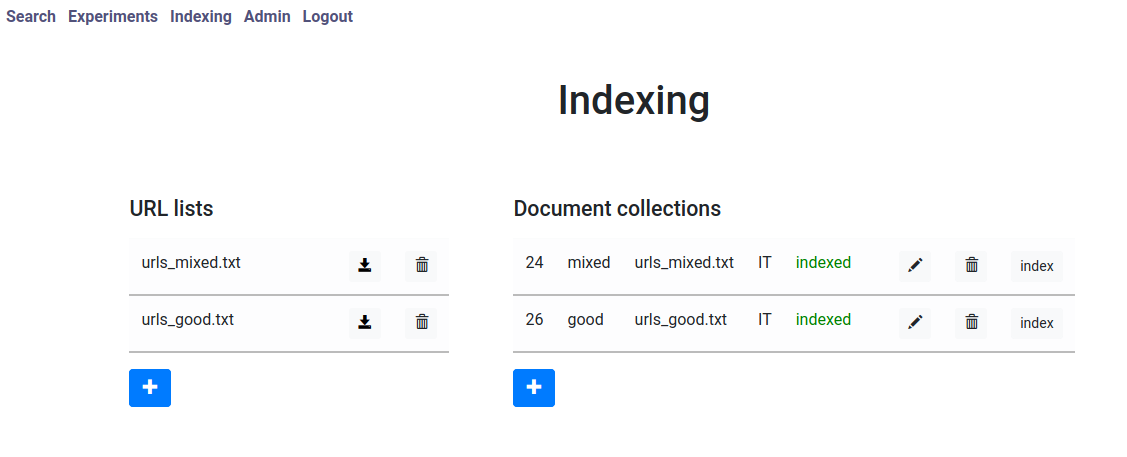
\includegraphics[width=0.9\textwidth]{img/indexingUi}
\caption{User interface for creating document collections}
\label{fig:indexingUi}
\end{figure}

\newpage


%%%%%%%%%%%%%%%%%%%%%%%%%%%%%%%%%%%%%%%%%%%
\subsection{Experiment Definition \small{(.../experiments/ui)}}

The \emph{/experiments/ui} page lists all defined experiments. Each line shows the experiment's unique id (needed for running
with a \emph{Qualtrics} survey, its title, mode (\emph{stand\_alone} or \emph{Qualtrics}), the assigned experimenter, the date on which it was defined, 
its status (one of \emph{created}, \emph{ready}, \emph{running}, or \emph{complete}), and buttons leading to the UI for configuration,
execution, and evaluation. The buttons are enabled or disabled depending on the experiment's status. \textbf{Figure \ref{fig:experimentsUi}}
shows the experiments interface.

\begin{figure} [h]
     \centering
     \begin{subfigure}[b]{0.8\textwidth}
         \centering
         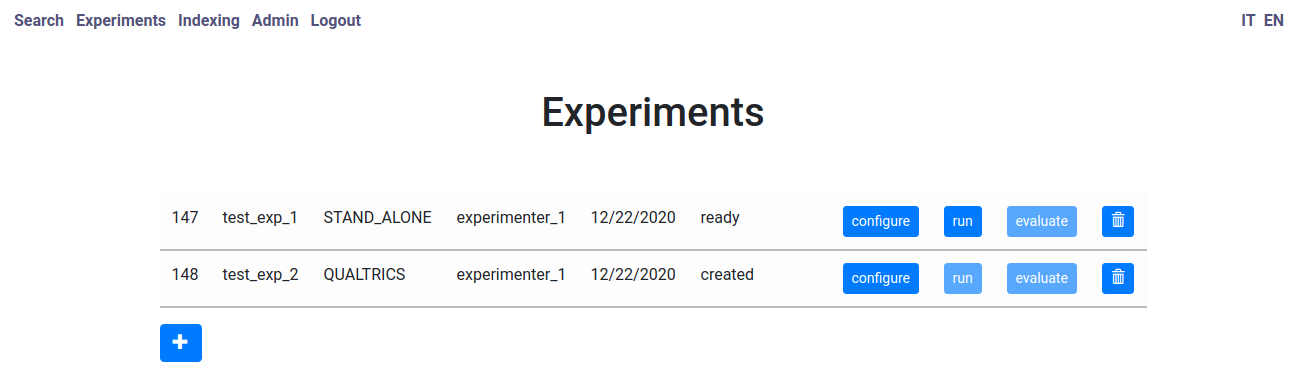
\includegraphics[width=\textwidth]{img/experiments_1}
         \caption{Experiments list}
         \label{fig:experimentsUi1}
     \end{subfigure}
     \par\bigskip
     \begin{subfigure}[b]{0.8\textwidth}
         \centering
         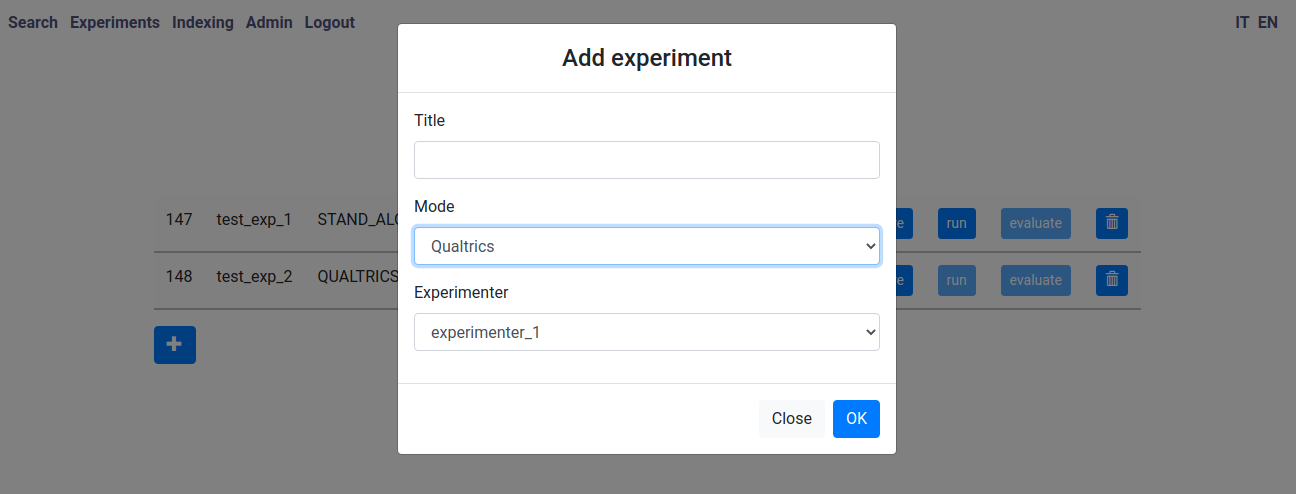
\includegraphics[width=\textwidth]{img/experiments_2}
         \caption{Popup for defining a new experiment}
         \label{fig:experimentsUi2}
     \end{subfigure}
     \caption{Interface for defining experiments}
     \label{fig:experimentsUi}
\end{figure}


%%%%%%%%%%%%%%%%%%%%%%%%%%%%%%%%%%%%%%%%%%%
\subsection{Experiment Configuration \small{(.../experiments/setup/ui)}}

The interface for experiment configuration is reachable by clicking on the \emph{configure} button in the
experiments list UI. If the experiment's mode is \emph{stand\_alone} the configuration involves creating test groups and assigning 
document collections and participants to them. Moreover a document collection can be set as predefined result list for the first query.
Participants and groups can be defined manually or loaded from a configuration file. If the mode is \emph{Qualtrics}, participants are created while
they take part in the survey.

\subsubsection{Configuration in stand-alone mode}

The setup UI for stand-alone experiments includes a section for uploading, inspecting, or deleting configuration files (which can be used for
defining test groups and participants), as well as a section for editing the test groups. \textbf{Figure \ref{fig:expSetupUi1}}
shows the page after two test groups have been added and edited; \textbf{Figure \ref{fig:expConfigFile}} shows an example of a configuration file. 
For the configuration to be complete, i.e. its status being set to 
\emph{complete} and the \emph{run} UI being available, there must be at least one test group defined, and each test group must 
have some participants and at least one document collection.

\begin{figure} [ht]
     \centering
     \hfill
     \begin{subfigure}{0.32\textwidth}
         \centering
         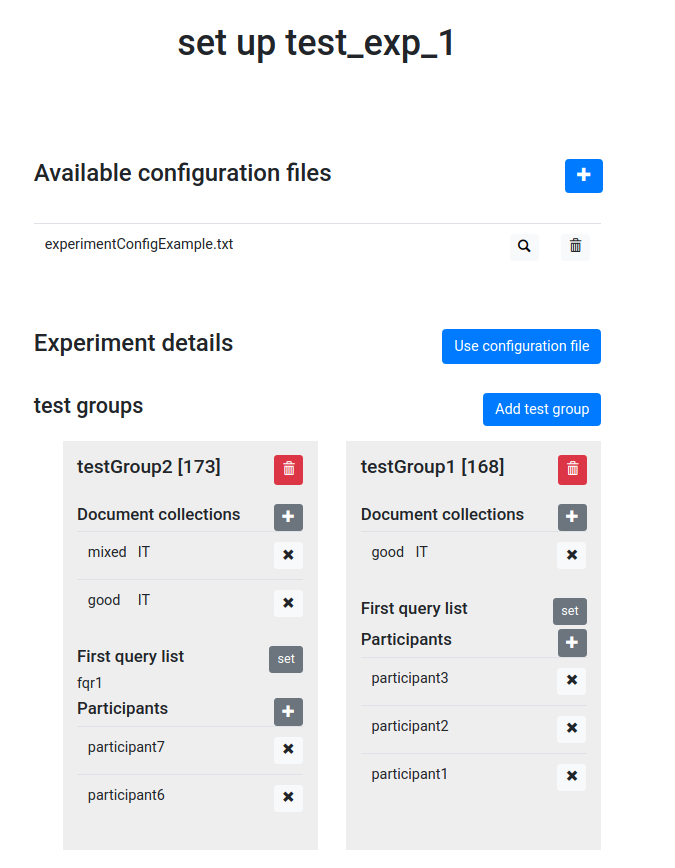
\includegraphics[width=\textwidth]{img/expSetup1}
         \caption{Experiment setup UI for stand-alone mode}
         \label{fig:expSetupUi1}
     \end{subfigure}
     \hfill
     \begin{subfigure}{0.5\textwidth}
         \centering
         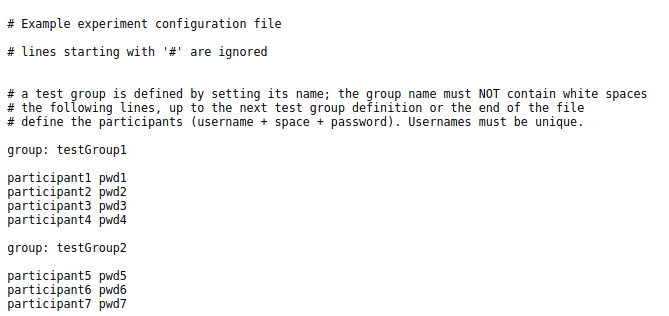
\includegraphics[width=\textwidth]{img/expConfigFile}
         \caption{Example of a configuration file}
         \label{fig:expConfigFile}
     \end{subfigure}
     \hfill
     \caption{}
     \label{fig:expConfigUi1}
\end{figure}

\newpage

\subsubsection{Configuration in Qualtrics mode}

In Qualtrics mode the setup options are similar, but the participants don't need to be specified, as they are defined during survey.
So the is no need for configuration files. For the configuration to be complete, there must be at least one test group, and each test group
must have at least one document collection. 

\textbf{Figure \ref{fig:expSetupUi2}} shows the configuration interface after creating and editing
two test groups. Notice the test group's id number: this will be needed when setting up the related Qualtrics survey. 

\begin{figure} [h]
\centering
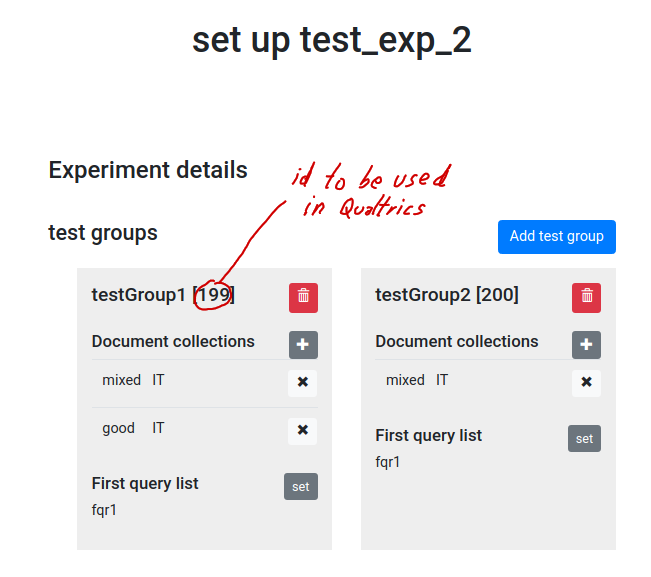
\includegraphics[width=0.5\textwidth]{img/expSetupUi2}
\caption{Experiment setup UI for Qualtrics mode}
\label{fig:expSetupUi2}
\end{figure}

\newpage

%%%%%%%%%%%%%%%%%%%%%%%%%%%%%%%%%%%%%%%%%%%
\subsection{Experiment Execution \small{(.../experiments/run/ui)}}

If an experiment is configured, the related execution UI becomes available. The interface is quite simple: there is a button
for starting, stopping and resetting the experiment, as well as live updated information on participants activities.
In stand-alone mode all participants are listed from the beginning, while in Qualtrics mode they appear as they log in.

The purpose of the start / stop mechanism is to enable participant access and to measure the experiment's duration. As
soon as the experiment is started, participants can lo in; when the experiment is stopped they are automatically logged out.
In case the experiment is defined in Qualtrics mode, the participants are redirected back to the survey.
After an experiment is started, the page can be left and returned to later.
\textbf{Figure \ref{fig:expRunUi}} shows the interface for running an experiment.

\begin{figure} [h]
\centering
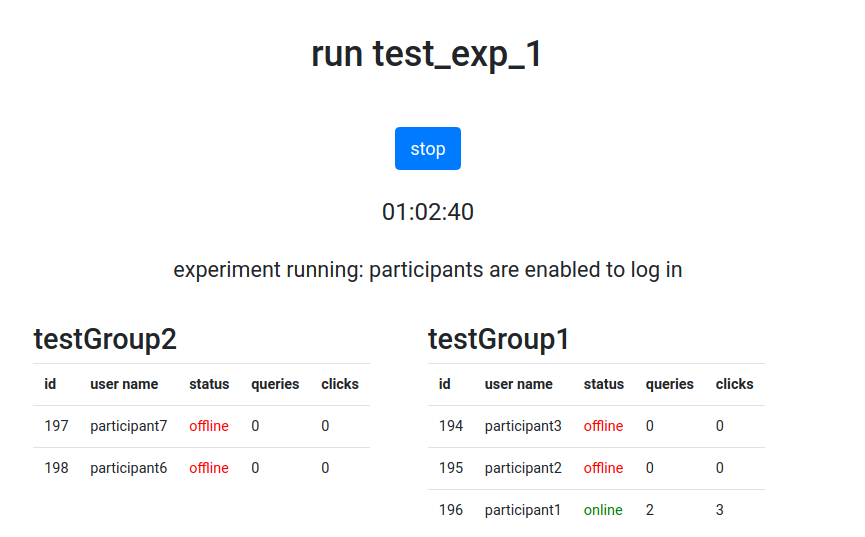
\includegraphics[width=0.5\textwidth]{img/expRunUi}
\caption{Experiments run UI}
\label{fig:expRunUi}
\end{figure}

%%%%%%%%%%%%%%%%%%%%%%%%%%%%%%%%%%%%%%%%%%%
\subsection{Setting up a linked Qualtrics survey}

For linking a survey to an experiment, the survey must contain
a block whose ``next'' button redirects to HSE, a failure block to be displayed in case accidentally the experiment is not running, or
there is some connection error,
and some settings at the beginning of the \emph{Survey flow}. 

\subsubsection{Survey Questions}

The redirection is set via \emph{JavaScript} in the survey question (see
\textbf{Figure \ref{fig:qualtricsLinkJs}}). The failure block needs no specific configuration.

\begin{figure} [h]
     \centering
     \hfill
     \begin{subfigure}[c]{0.3\textwidth}
         \centering
         
\includegraphics[width=\textwidth]{img/qsl1}
         \caption{Opening the JS editor}
         \label{fig:qsl1}
     \end{subfigure}
     \hfill
     \begin{subfigure}[c]{0.35\textwidth}
         \centering
         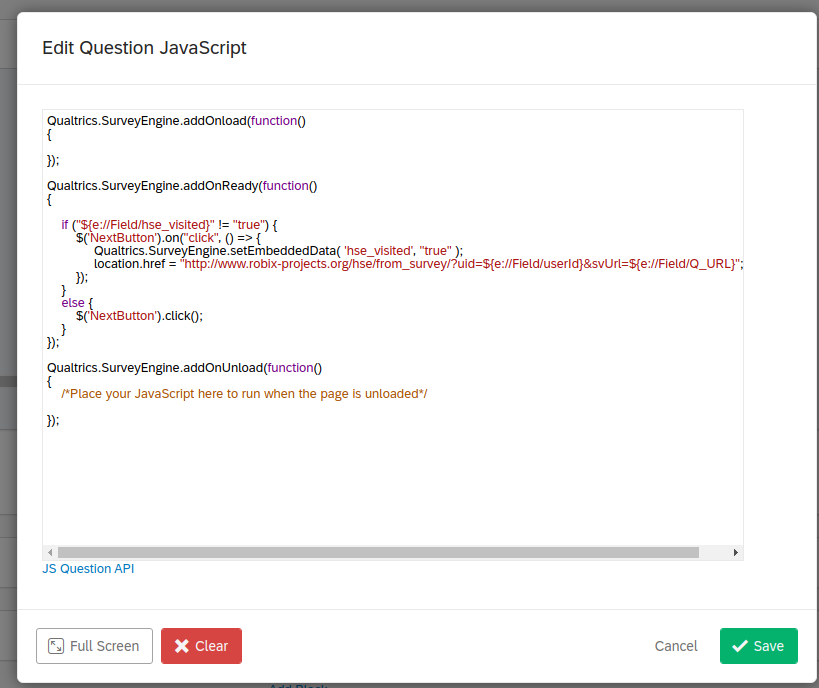
\includegraphics[width=\textwidth]{img/qsl2}
         \caption{Edited JS}
         \label{fig:qsl2}
     \end{subfigure}
     \hfill
     \caption{}
     \label{fig:qualtricsLinkJs}
\end{figure}

In the JS editor there are three default functions: \texttt{Qualtrics.SurveyEngine.addOnload(...)}, \texttt{Qualtrics.SurveyEngine.addReady(...)},
and \texttt{Qualtrics.SurveyEngine.addOnUnload(...)}. The first and third functions don't need to be modified, while the
\texttt{Qualtrics.SurveyEngine.addReady(...)} function needs to be edited as follows:


\begin{verbatim}
Qualtrics.SurveyEngine.addOnReady(function()
{
    if ("${e://Field/hse_visited}" != "true") {

        $('NextButton').on("click", () => {
            Qualtrics.SurveyEngine.setEmbeddedData( 'hse_visited', "true" );
            location.href = "http://[hse server url]/from_survey/ 
                             ?uid=${e://Field/userId}&svUrl=${e://Field/Q_URL}";				   
        });
    }
    else {

        $('NextButton').click();					  
    }					  
});
\end{verbatim}

\subsubsection{Survey Flow}

The following elements are to be added at the beginning of the survey flow, in the order thea are presented here:

\begin{enumerate}

\item
    An \emph{Embedded Data} element for initializing some variables:

    \begin{figure} [h]
    \centering
    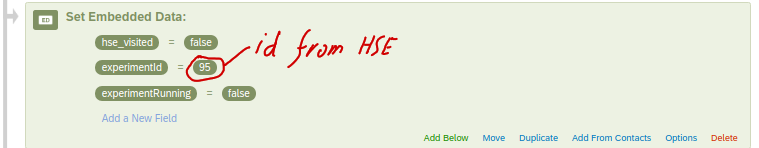
\includegraphics[width=.9\textwidth]{img/qflow1}
    \label{fig:qflow1} 
    \end{figure}

\item
    A \emph{Web Service} element to do an API call for checking that the given experiment is actually running:

    \begin{figure} [h]
    \centering
    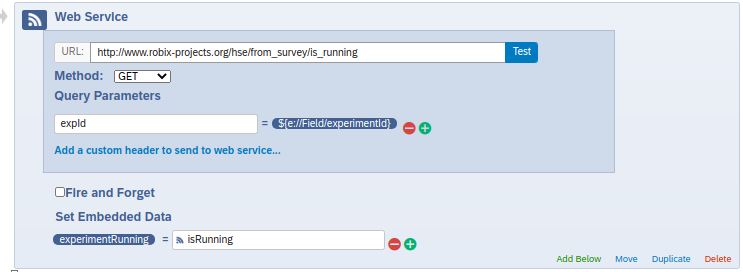
\includegraphics[width=.9\textwidth]{img/qflow2}
    \label{fig:qflow1} 
    \end{figure}

\newpage

\item
    A \emph{Branch} element to interrupt the survey if the experiment is not running:

    \begin{figure} [h]
    \centering
    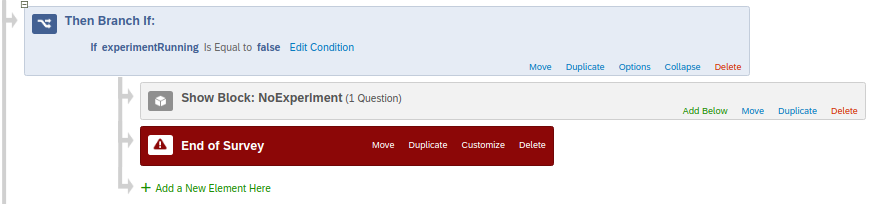
\includegraphics[width=.9\textwidth]{img/qflow3}
    \label{fig:qflow1} 
    \end{figure}

\item
    A \emph{Randomizer} element for assigning participants to test groups:

    \begin{figure} [h]
    \centering
    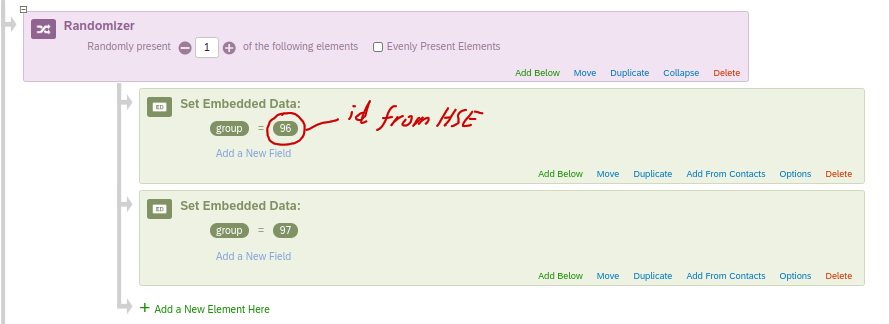
\includegraphics[width=.9\textwidth]{img/qflow4}
    \label{fig:qflow1} 
    \end{figure}

\item
    A \emph{Web Service} element for initializing the participant in HSE:

    \begin{figure} [h]
    \centering
    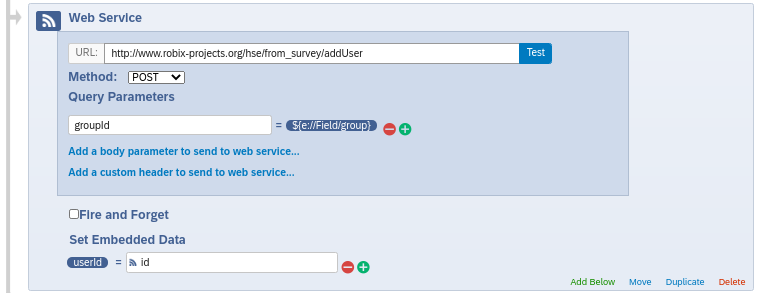
\includegraphics[width=.9\textwidth]{img/qflow5}
    \label{fig:qflow1} 
    \end{figure}

\end{enumerate}

\vspace{.5cm}

\textbf{Figure \ref{fig:qflow}} on the next page shows the entire edited survey flow.

\begin{figure} [h]
\centering
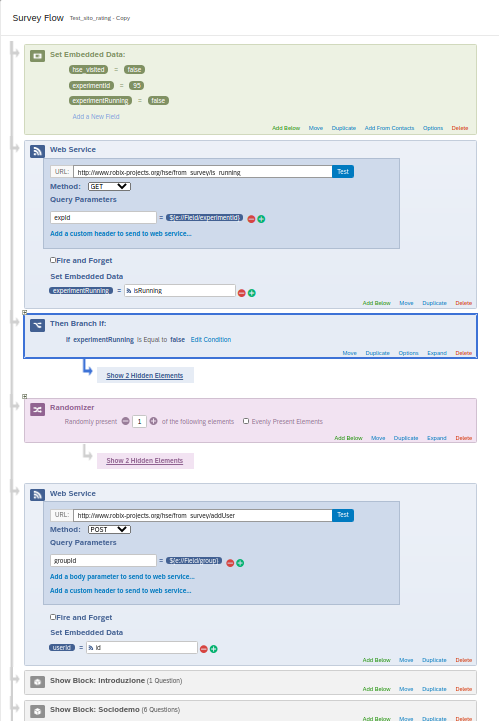
\includegraphics[width=\textwidth]{img/qflow}
\caption{Edited Survey Flow}
\label{fig:qflow}
\end{figure}














\end{document}















